%%%%%%%%%%%%%%%%%%don't forget if needed %%%%%%%%%%%%%%%%%%%%%
%\section[toc version]{title version%
%              \sectionmark{head version}}
%\sectionmark{head version}
%%%%%%%%%%%%%%%%%%%%%%%%%%%%%%%%%%%%%%%%%%%%%%%%%%%%%%%%%%%%%%
\def\titcourt{Numerical simulation of melting of phase change materials heated from below}
\def\titlong{Numerical simulation of melting of phase change materials heated from below}
%%%%%%%%%%%%%%%%%%%%%%%%%%%%%%%%%%%%%%%%%%%%%%%%%%%%%%%%%%%%%%%%
\chapter[\titlong]{\titlong%
              \chaptermark{\titcourt}}
\chaptermark{\titcourt}
\label{chap-MELTING-BELOW}
%%%%%%%%%%%%%%%%%%%%%%%%%%%%%%%%%%%%%%%%%%%%%%%%%%%%%%%%%%%%%%%%
%%%%%%%%%%%%%%%%%%%%%%%%%%%%%%%%%%%%%%%%%%%%%%%%%%%%%%%%%%%%%%%%

The melting of PCM heated from the side was presented in Sec. \ref{chap-MELTING}.
The dynamic of the melting, the identification of three regimes describing the melting process and the effect of the Rayleigh number have been discussed in detail.
In this chapter, we pay more attention to PCM heated from below.
This configuration is indeed known to be overspread in the nature or in human activities, such as geophysical flows (Earth's mantle formation, magma oceans) or heat dissipation from electronic devices.

While the melting of PCM heated from the side have attracted many consideration, the melting of PCM heated from below have received less attention.
\cite{diaz1984visualization,hale1980solid} have studied experimentally the solid-liquid interface morphology of PCM during basal heating.
\cite{gong1998flow} studied numerically the flow and heat transfer during the melting of pure n-octadecane in a rectangular cavity heated from below.
Recent numerical simulations investigate different boundary conditions such as
periodic configurations along the horizontal axis \citep{esfahani2018basal,madruga2018dynamic,favier2019rayleigh} or wavy surface in a rectangular cavity heated from below \citep{kousksou2014melting}.

 We investigate in this chapter the melting of a pure octadecane PCM in a square enclosure heated from below.
 The dynamics of the melting is fundamentally different in the basal heating case compared with the lateral heating.
 It has been observed that for this configuration natural convection develops in the form of Benard cells and
 results in a nonplanar solid-liquid interface. 
\citep{vasil2011dynamic,favier2019rayleigh} have studied the hydrodynamic instabilities at the onset of convection and compared their observation with the classical Rayleigh-B�nard \citep{chandrasekhar2013hydrodynamic} instability mechanism.
\citep{favier2019rayleigh} have focused their attention to the effect of the non-planar topography of the interface to the convection flow.
 On the other hand, \citep{gong1998flow,esfahani2018basal,madruga2018dynamic} mostly focused on global quantities such as the heat flux and the statistical properties of the interface.

The physical parameters considered are the same as presented in Sec. \ref{sec-melting}:
$\Pr = 56.2$ and $\Ste = 0.045$.
Three Rayleigh numbers are carried out: $\Ray = 3.27 \cdot 10^5$, $\Ray = 1.62 \cdot 10^6$, $\Ray = 3.27 \cdot 10^6$ to assess the influence of the size of the domain on the dynamic of the natural convection flow
as observed by \cite{madruga2018dynamic}.
The PCM is initially solid at a cold dimensionless temperature $\theta_c$ under the temperature of fusion.
The top of the wall is set at an isothermal temperature $\theta = \theta_c$, the vertical wall are adiabatic and the bottom is heated at a dimensionless temperature $\theta = \theta_h$.
 We carried out a two-dimensional numerical simulation even if 
 \cite{gau1983flow} and  \cite{gong1998flow} have noticed the existence of three-dimensional convection cells during the very first step of the melting process.
 Indeed, this three-dimensional convection cell can be neglected since the duration is very short compared with the whole melting step,
so that the two-dimensional model is realistic.
A qualitative observation of the dynamic of the natural convection flow and its impact on the melting front is first addressed.
Second, the observation of four regimes during the melting is discussed.
Finally, a comparison between the lateral and the basal heating is presented.

\section{Time evolution of the melting process} \label{sec-RB-melt-process}

The natural convection flow in the melt PCM during lateral heating exhibits convection cells deforming the solid-liquid interface (see Fig. \ref{fig:melt-field}).
The dynamic of the natural convection flow during the basal heating is fundamentally different.
It is well known that any non-planar topography can lead to a baroclinic flow at any Rayleigh number.

Fig. \ref{fig:melt-below} displays the structure of the natural convection in the melt PCM through a sequence of panels for temperature isolines and streamlines in the liquid phase.
An array of lengthening plumes (panel a to c) and counter-rotating convective cells (panel d to f)  is located in the liquid phase.
The number of convective cells and plumes increases with the Rayleigh number.
For $\Ray = 3.27 \cdot 10^5$, three equidistant plumes (Fig. \ref{fig:melt-below}a) and five convective cells (Fig. \ref{fig:melt-below}d) can be observed, while four and six plumes are observed for $\Ray = 1.62 \cdot 10^6$ and $\Ray = 3.27 \cdot 10^6$ respectively (Figs. \ref{fig:melt-below}b and \ref{fig:melt-below}c).
These observations agree well with the numerical results of \cite{gong1998flow} and \cite{madruga2018dynamic}.

The shape of the interface is directly linked to the dynamic of the plumes.
The mushroom form of the plumes results from the two symmetric counter-rotating convective cells surrounding each plumes.
We observe an anti-clockwise recirculation of the left convection cell and a clockwise recirculation of the right.
Thus, the melt is heated to the highest temperature at bottom and then floats up, reaches the phase change interface and splits into opposite directions.
The melt is cooled as it flows through the phase change interface.
It results a non-planar interface with a peak at the center of each couple of counter-rotating convective cells.
\begin{figure}
	\begin{center}
		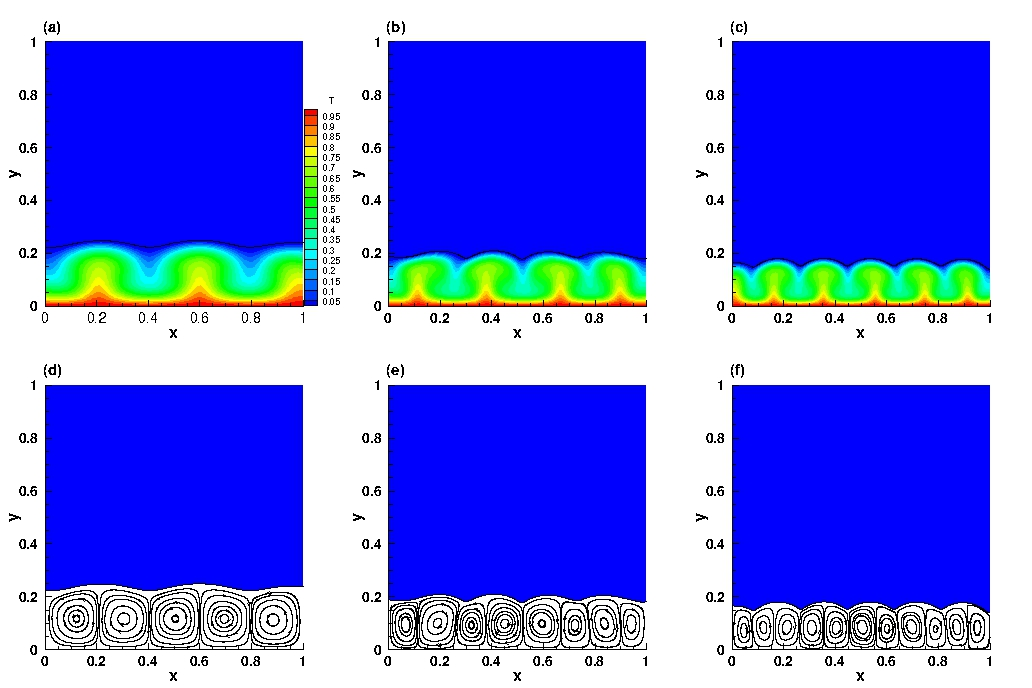
\includegraphics[width=\textwidth]{\figpath/Fig_cap_melting_basal/T_MELT_BASAL_heating_2}
	\end{center}
	\caption{Melting of PCM heated from below: Temperature field and solid-liquid interface for different size of the domain. (a) $\Ray = 3.27 \cdot 10^5$ and $t=30$, (b)  $\Ray = 1.62 \cdot 10^6$ and $t=15$, (c) $\Ray = 3.27 \cdot 10^6$ and $t=10$.}
	\label{fig:melt-below}
\end{figure}

It is useful to introduce the effective Rayleigh and Nusselt numbers of the fluid layer, based on the height of the melting PCM, to describe the temporal evolution of the melting:

\begin{eqnarray}
	Ra_{e} &=& Ra \times \bar {\delta_H}^3, \\
	N\!u_{e} &=& N\!u \times \bar{\delta_H},
\end{eqnarray}
with $\bar{\delta_H}$ the averaged fluid height. Note that $\bar{\delta_H}$ here can be assimilated to the liquid fraction.
In the limit of vanishing $\Ste$ number, the classical no-slip Rayleigh-B�nard convection predicts a critical Rayleigh number $\Ray_c \approx 1707.76 $ \citep{chandrasekhar2013hydrodynamic} after which the first instability appears and the melting front becomes non-planar.
This critical value is increased for increasing values of $\Ste$.
In our simulations, the convective onset occurs at around $\Ray_e \approx 3 \times 10^3$, which is in good agreement with the observation of \citep{esfahani2018basal,favier2019rayleigh}.

\begin{figure}
	\begin{center}
		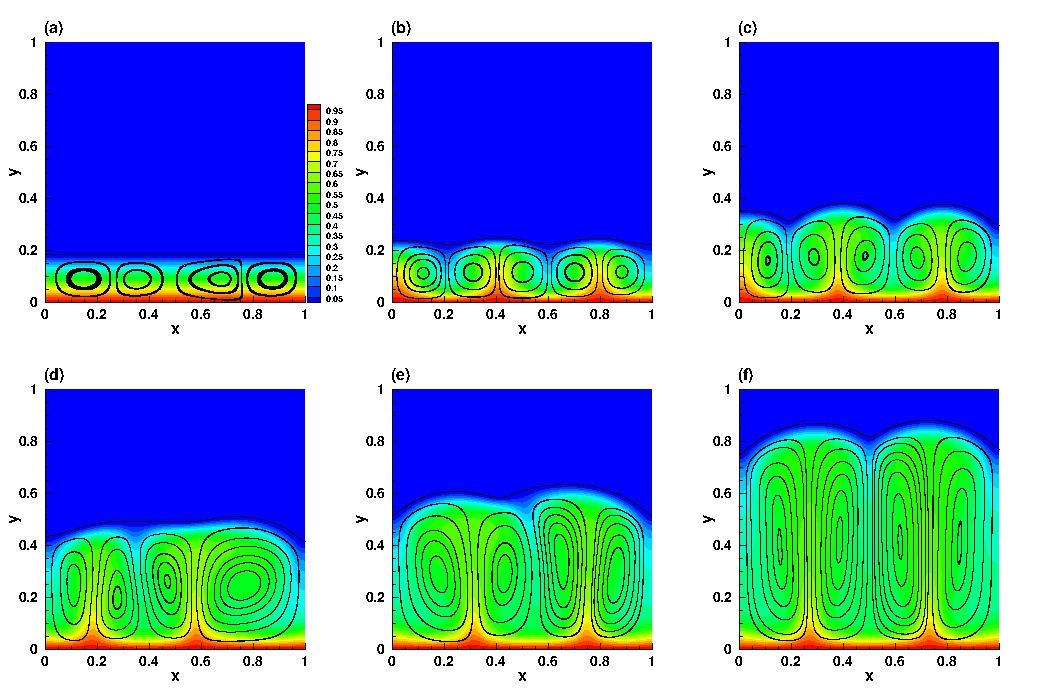
\includegraphics[width=\textwidth]{\figpath/Fig_cap_melting_basal/T_evol_Ra-327e5}
	\end{center}
	\caption{Melting of PCM heated from below: Temperature field and solid-liquid interface for different size of the domain. (a) $\Ray = 3.27 \cdot 10^5$ and $t=30$, (b)  $\Ray = 1.62 \cdot 10^6$ and $t=15$, (c) $\Ray = 3.27 \cdot 10^6$ and $t=10$.}
	\label{fig:T-evol-Ra-3.27e5}
\end{figure}

The time evolution of the melting for $\Ray = 3.27 \times 10^5$ is illustrated in details in Fig. \ref{fig:T-evol-Ra-3.27e5} in panels (a) to (f).
Before the first instability arise, the melt layer evolves solely by conduction. 
There is no noticeable fluid flow and the melting front remains straight (panel (a)).
The convective onset occurs at around $\Ray_e \approx 3 \times 10^3$ and the phase-change interface becomes non-planar (panel (b)).
The appearance of convection is marked by a change in the shape of the interface from straight to nearly periodic curve.
While the fluid depth increases, the effective Rayleigh number increases and the convective rolls are stretched vertically (panels (b) and (c)).
We note that during this stage, the number of rolls is time-independent.
This stage can be compared to the steady convection after the onset in the Rayleigh-B�nard system.
After the rolls are elongated vertically, they start to oscillate laterally and then merge to create greater rolls (panels (d) and (e)).
The essential consequence of the foregoing observation is that the melting front is modified.
The interface is actually shaped by the new flow pattern. 
Two peaks are observed but is still periodic at the interface related to the four convective rolls.
The foregoing steady convection observation is then observed again after the rolls have merged (panel (f)).

\begin{figure}
	\begin{center}
		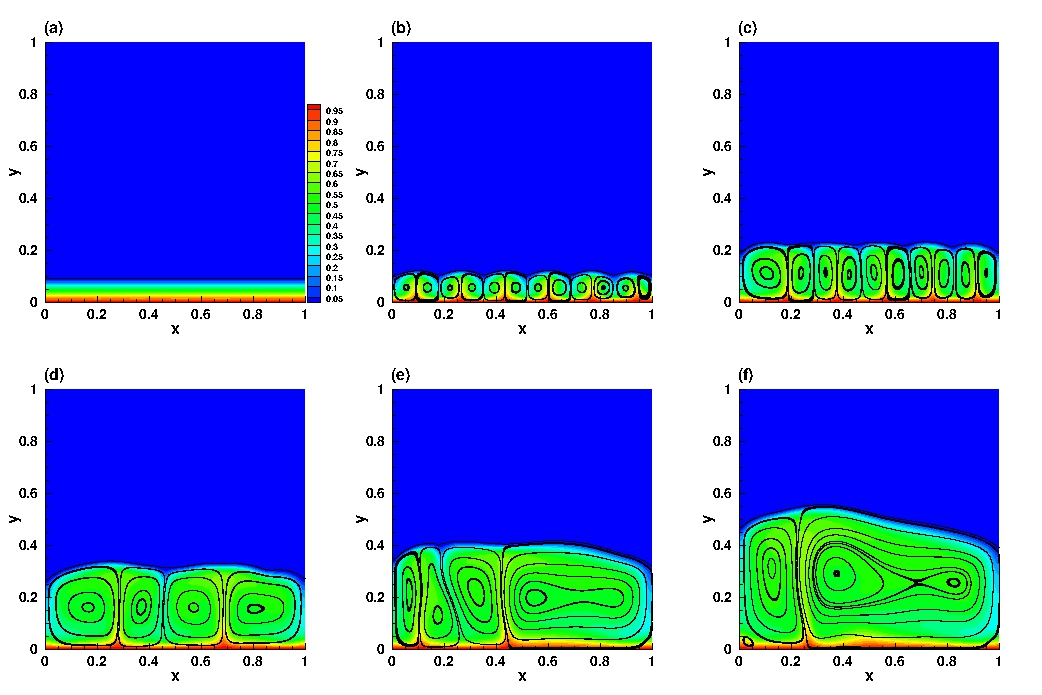
\includegraphics[width=\textwidth]{\figpath/Fig_cap_melting_basal/T_evol_327e6_1}
		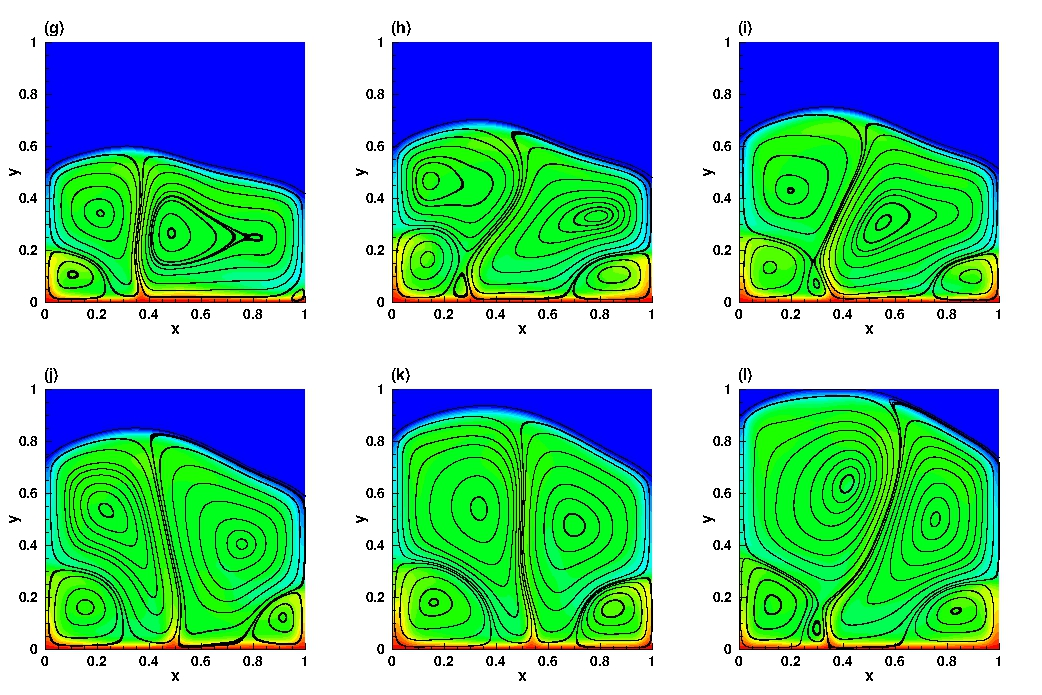
\includegraphics[width=\textwidth]{\figpath/Fig_cap_melting_basal/T_evol_327e6_2}
	\end{center}
	\caption{Melting of PCM heated from below: Temperature field and solid-liquid interface for different size of the domain.$\Ray = 3.27 \cdot 10^6$}
	\label{fig:T-evol-Ra-3.27e6}
\end{figure}

Fig. \ref{fig:T-evol-Ra-3.27e6} shows the dynamic of the melting for higher $\Ray$ number.
The size of the cavity is increased of an order of three, corresponding to $\Ray = 3.27 \times 10^6$ while the $\Ste$ number remains the same.
The stages described previously are recovered in panels (a) to (d).
At $\Ray_e = 4 \times 10^5$ the interface loses periodicity and becomes smoother without cusps (panels (e) and (f)).


\begin{figure}
	\begin{center}
		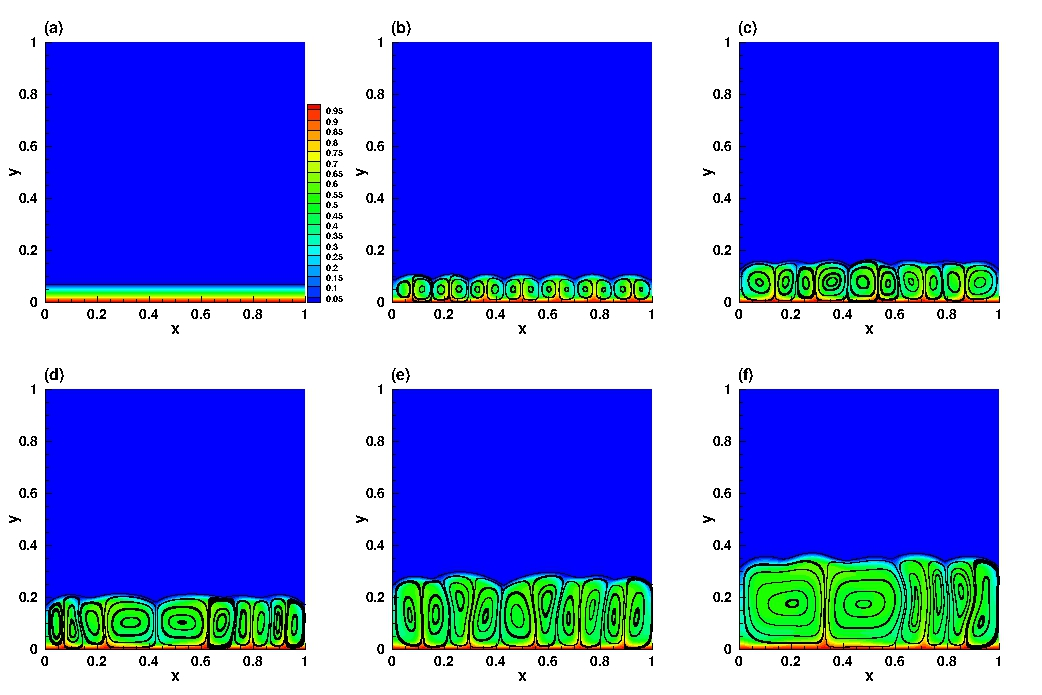
\includegraphics[width=\textwidth]{\figpath/Fig_cap_melting_basal/T_evol_654e6_1}
		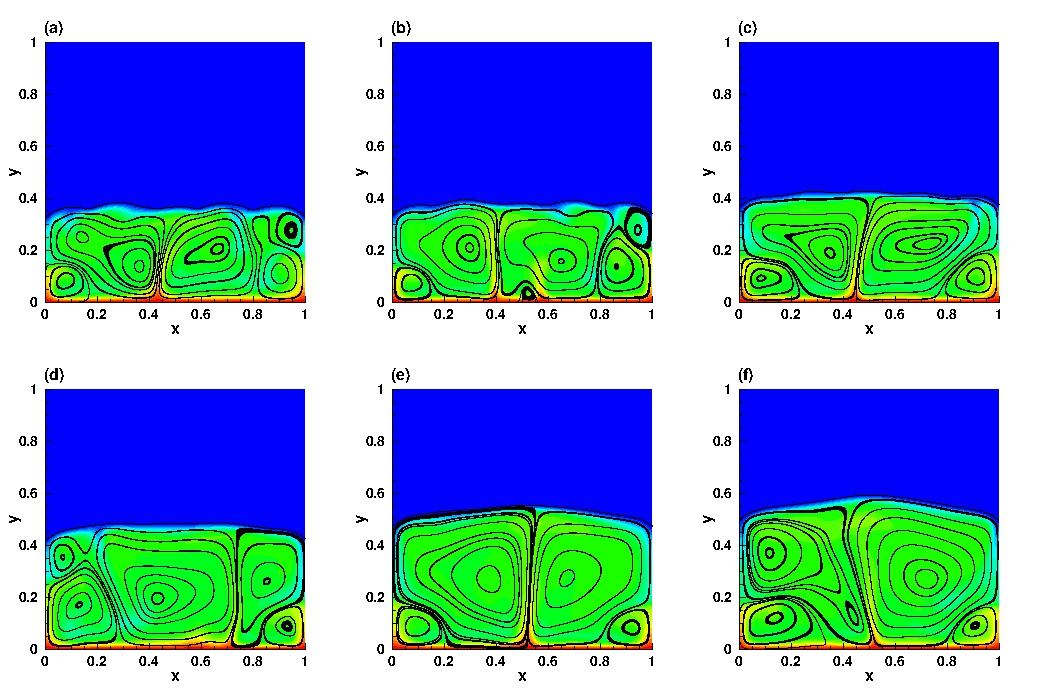
\includegraphics[width=\textwidth]{\figpath/Fig_cap_melting_basal/T_evol_654e6_2}
	\end{center}
	\caption{Melting of PCM heated from below: Temperature field and solid-liquid interface for different size of the domain. (a) $\Ray = 3.27 \cdot 10^5$ and $t=30$, (b)  $\Ray = 1.62 \cdot 10^6$ and $t=15$, (c) $\Ray = 3.27 \cdot 10^6$ and $t=10$.}
	\label{fig:T-evol-Ra-6.54e6}
\end{figure}

\section{Scaling analysis} \label{sec-RB-scal-analysis}

The previous observation can be assessed more quantitatively by evaluating the heat transfert rate during the melting.
Fig. \ref{fig:NU-LF-evol} plots the temporal evolution of $N\!u_e$ when the melting evolve, i.e. when the $\Ray_e$ increases.
The onset of the convection arises at $\Ray_e = 3 \times 10^3$ when a sudden jump in $N\!u_e$ is observed.
\cite{vasil2011dynamic} have investigated a weakly non-linear stability analysis and have highlighted a superexponentional amplitude growth when the Rayleigh number becomes close to the traditional critical value in the limit of vanishing Stefan number.
This superexponential growth is followed by a rapid pattern readjustment.
The trend of $N\!u_e$ at the onset of convection is in total accordance with the foregoing prediction of \cite{vasil2011dynamic}.

\begin{figure}
	\begin{center}
		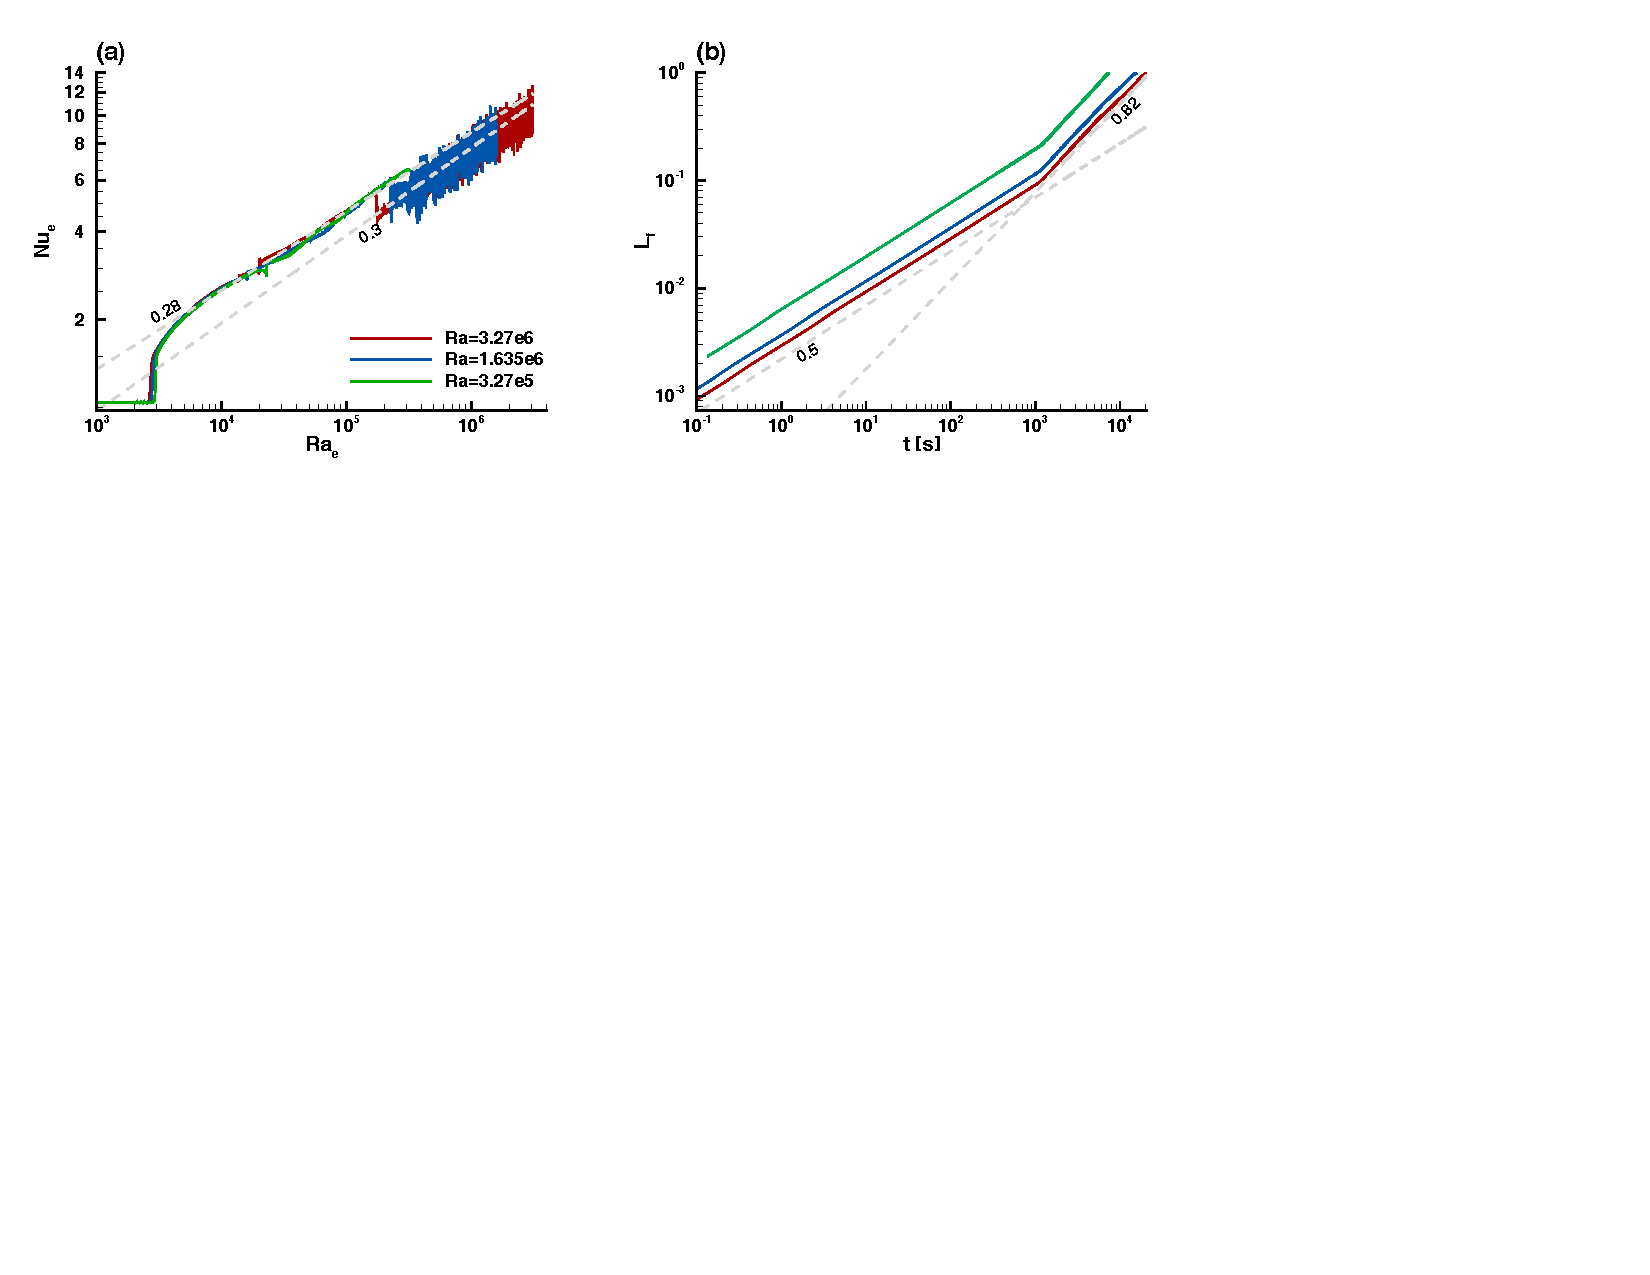
\includegraphics[width=\textwidth]{\figpath/Fig_cap_melting_basal/NU-LF-PHYS}
	\end{center}
	\caption{Melting of PCM heated from below: Temperature field and solid-liquid interface for different size of the domain. (a) $\Ray = 3.27 \cdot 10^5$ and $t=30$, (b)  $\Ray = 1.62 \cdot 10^6$ and $t=15$, (c) $\Ray = 3.27 \cdot 10^6$ and $t=10$.}
	\label{fig:NU-LF-evol}
\end{figure}
